\chapter{Evaluation}
\label{chap:eval}
In diesem Kapitel wird die entstandene Implementierung gegen die Anforderungen verglichen und das Ergebnis evaluiert.

\section{Erfüllte Ziele}
Alle formalen Anforderungen, wie sie in Sektion \ref{sec:anforderungen} festgehalten sind, wurden erfüllt. Der Demonstrator läuft on-premise auf dem Raspberry Pi und verwaltet sämtliche Daten lokal. Es ist möglich komplexe Szenarien zu definieren, wobei intelligente Geräte mit Webdiensten frei zusammengefügt werden können. Dies ist möglich, da die integrierten Webservices ebenfalls als \textit{Things} im System abgebildet sind. Schließlich ist eine Benutzeroberfläche vorhanden, die es dem Nutzer erlaubt zur Laufzeit neue Szenarien zu erstellen, zu editieren und zu löschen.

\section{Vergleich mit Smart Home}
Bei dem entwickelten Demonstrator handelt es sich um eine typische Smart Home Lösung, die auf \textit{Eclipse SmartHome} basiert und um weitere Funktionalitäten angereichert wurde. Dadurch besitzt er alle üblichen Funktionalitäten, die ein Smart Home enthält - er ist in der Lage ausgewählte intelligente Geräte direkt anzusteuern und in Szenarien zu automatisieren. 

\section{Vergleich mit IFTTT}
Es ist zu beachten, dass es sich bei IFTTT um einen Cloud-Service handelt. Dadurch hat es keine Möglichkeit intelligente Geräte im Haus zu steuern, sofern diese nicht über eine vom Hersteller bereitgestellte Webschnittstelle verfügen.

In IFTTT ist es nur möglich simple Szenarien auf eine einfache Art und Weise zu definieren. Hierbei handelt es sich um sogenannte \glqq if this than that\grqq{} Szenarien, die über jeweils nur einen Trigger (\glqq this\grqq) und eine Action (\glqq that \grqq) verfügen. Der Demonstrator hingegen erlaubt es komlexe ECA-Regeln zu definieren.

Der entstandene Demonstrator wurde einem umfassenden Test unterzogen, im Laufe dessen Durchsatz und Reaktionszeiten gemessen und mit IFTTT verglichen wurden. 

\subsection{Kopieren von Dateien in der Dropbox}
Um Durchsatz zu messen, wurde ein Szenario definiert, dass sämtliche Dateien, die in einen bestimmten Ordner in Dropbox hinzugefügt wurden, in einen anderen Ordner in der Dropbox zu kopieren. Zu Beachten ist, dass IFTTT sich auf die Abarbeitung von bis zu 15 Dateien pro Abfrage begrenzt und Dateien, die größer, als 30MB sind, nicht beachtet. Zusätzlich wird vom Service gewarnt, dass die Ausführung aller Szenarien sich um bis zu 1 Stunde verzögern kann.
Es wurde geprüft, wie gut die beiden Anwendungen mit einer großer Anzahl kleiner Dateien, sowie mit geringer Anzahl von großen Dateien umgehen können. 

\subsubsection{Zahlreiche kleine Dateien}
Es wurden Mengen von 258KB großen Dateien gleichzeitig in einen Dropbox Ordner hochgeladen. Es wurden jeweils Vielfache von 15 verwendet, da dies die maximale Anzahl von Dateien ist, die IFTTT in einer Abfrage bearbeitet.

Es entstanden die Grafiken \ref{fig:eval1} und \ref{fig:eval2}.
\begin{figure}
	\centering
	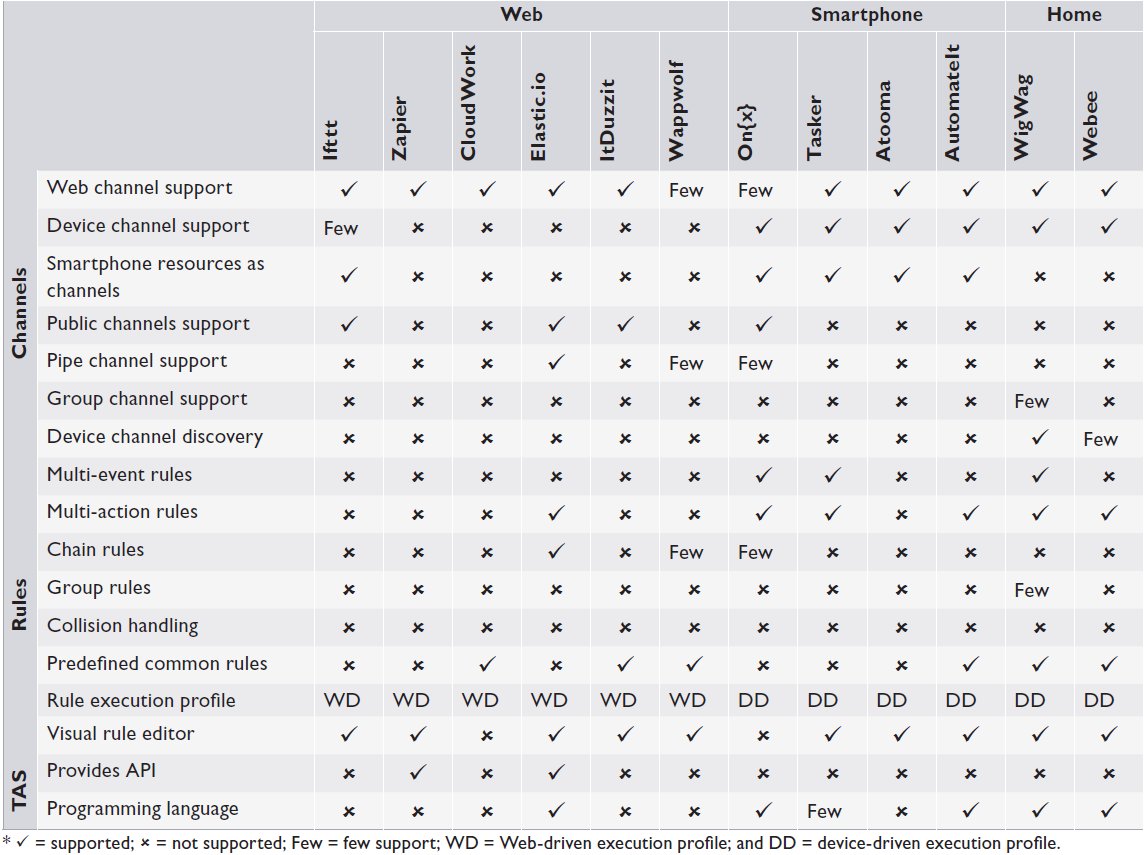
\includegraphics[width=\textwidth]{bilder/TASOverview}
	\caption{Here will be another image}
	\label{fig:eval1}
\end{figure}

\begin{figure}
	\centering
	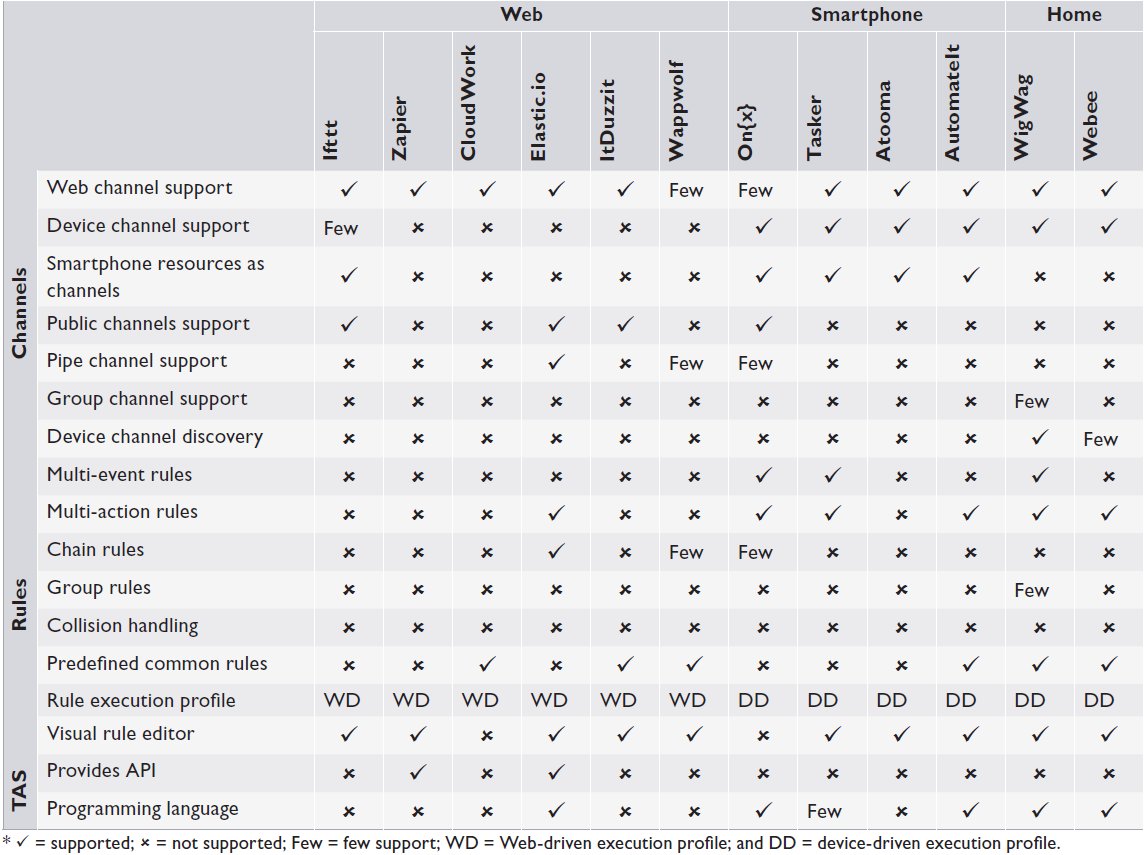
\includegraphics[width=\textwidth]{bilder/TASOverview}
	\caption{Here will be another image}
	\label{fig:eval2}
\end{figure}

Für die Erstellung von Grafik \ref{fig:eval1} wurde für jede hochgeladene Datei einzeln gemessen, wie viele Sekunden es dauert, bis eine Kopie im Zielordner vorhanden ist. Es wurde anschließend ein Mittelwert gebildet und die Messung mehrmals wiederholt. Schließlich wurde ein gemeinsamer Mittelwert über die gesammelten Werte gebildet und in der Grafik für die verschiedenen Mengen von Dateien dargestellt.

In der Grafik \ref{fig:eval2} wurde analog gehandelt, mit dem Unterschied, dass hier dargestellt ist, was die längste Dauer zwischen hochladen einer Datei und der Bereitstellung der Kopie ist.

\subsubsection{Große Dateien}
IFTTT ist in der Lage mit Dateien umzugehen, die bis zu 30MB groß sind. Eine Wiederholung der oben genannten Messung mit 25MB großen Dateien hat ergeben, dass sich die Ergebnisse  analog verhalten. 

Der Demonstrator ist in der Lage mit Dateien \glqq beliebiger\grqq Größe umzugehen. Im Test gab es auch bei Verschiebung von 300MB großen Dateien keinerlei Probleme.

\subsection{Steuern von Lampen bei Tweets}
Es wurde sowohl auf IFTTT als auch auf dem Demonstrator ein Szenario erstellt, dass bei jedem Tweet eine Philips Hue Lampe ausschaltet. Anschließend wurde gemessen, wie lange es dauert, bis die Lampe tatsächlich ausgeschaltet wird, nachdem der Tweet veröffentlicht wurde. 

Es hat sich ergeben, dass die Reaktionszeit des Demonstrators stets unter einer Sekunde lag, während die Schaltung durch IFTTT eine sehr variable Dauer aufwies. Die schnellste Reaktionszeit lag bei ungefähr 10 Sekunden.


\subsection{Auswertung}
Aus den Messungen hat sich gezeigt, dass der Demonstrator IFTTT in jeder Hinsicht deutlich voraus ist. Dadurch, dass er sich im Hause des Nutzers befindet, ist er in der Lage Geräte direkt anzusteuern...

\section{Quellcode}

\section{Fazit}
